\documentclass[11pt]{article}
\usepackage[utf8]{inputenc}
\usepackage{amsmath}
\usepackage{graphicx}
\usepackage[top=1.55cm, bottom=2.29cm, left=1.6cm, right=1.47cm]{geometry}
\usepackage{fancyhdr}

% Initial pararagraph blankspace
\makeatletter 
\renewcommand{\paragraph}{\@startsection{paragraph}{4}{\z@}{-3.25ex \@plus 
-1ex \@minus -.2ex}{1.5ex \@plus .2ex}{\normalfont\normalsize\bfseries}} 
\makeatother

% Makes figures stay in place:
\usepackage{float}

\usepackage{parskip}
\setlength{\parindent}{15pt}

\begin{document}

%%%% FRONTPAGE %%%%%%%%%%%%%%%%%%%%%%%%%%%%%%%%%%%%%%%%%%%%%%%%%%%%%%%%%%%
\begin{center}

\includegraphics[width=0.25\textwidth]{images/uc3m.jpg}\\[2cm]
\textsc{\LARGE Universidad Carlos III de Madrid}\\[0.5cm]
\textsc{\Large Perception Systems}\\[4cm]


% Title
{\huge \bfseries{GECKO\\Gesture Recognition}\\[8cm]}


% Author and supervisor
\begin{minipage}{0.55\textwidth}
\begin{flushleft} \large
\emph{Authors:}\\
David Estévez Fernández (100282441)\\
Irene Sanz Nieto (100282826)\\
\end{flushleft}
\end{minipage}
\begin{minipage}{0.4\textwidth}
\begin{flushright} \large
\emph{Teacher:}\\
Abdulla Hussein Abdulrahm Al Kaff
\end{flushright}\end{minipage}\vfill

% Bottom of the page
{\large \today}

\end{center}
%
\newpage
%
%%%%%%Table of contents%%%%%%%%%%%%%%%%%%%%%%%%%%%%%%
%%%%%%%%%%%%%%%%%%%%%%%%%%%%%%%%%%%%%%%%%%%%%%%%%%%%%
\tableofcontents
\newpage

% Style
\lhead{}
\chead{}
\rhead{GECKO: Gesture Recognition}
\pagestyle{fancy}

%%%%% Includes %%%%%%%%%%%%%%%%%%%%%%%%%%%%%%%%%%%%%%%
%%%%%%%%%%%%%%%%%%%%%%%%%%%%%%%%%%%%%%%%%%%%%%%%%%%%%%
\section{Introduction}
In this document a gesture recognition software named GECKO is presented. This software will allow the user to interact with a computer using just hand gestures. 

For the software development we used a version control system based on git, and stored the code on the following online repository:

\begin{center}
{\bfseries https://github.com/David-Estevez/gecko}
\end{center}
~\\
\noindent
The code is released under a GPLv3 license, for anyone to download, study and improve our code.

\subsection{Motivation}
The necessity of doing a software for this subject (Systems of perception) gave us the opportunity to have a deeper knowledge of the theory of the course and of the OpenCV libraries. The first thing that was clear was that the software developed should be useful, and not only implement the theoretical concepts but also have an utility afterwards. That is how the idea of developing a gesture recognition system appeared. 

Also, the possibility of extending this software in the future to different machines (not only computers but also robots with webcams) was a great motivation in doing the whole project. 


\subsection{First Steps}

The first approach was to make a color segmentation (using the HSV color space) and select the hand using the size of the contour. Once the hand was detected, it was possible (after pressing a key) to move the mouse with the hand. The control was not very accurate due to the different problems present in the system such as illumination changes or having parts of the palm and fingers with a color outside the selected skin color range. In this first approach, it was possible to select between the theoretical values and the custom values obtained by placing the hand inside a square and getting automatically the skin HSV range. 

The theoretical skin range worked better than the custom range, but the poor segmentation caused a fluctuant output image. This did not allow to obtain a good gesture recognition.   

In order to better the hand's position and orientation estimation, two kalman filters were implemented. Those filters allowed a moderatedly accurate mouse control, if the background did not interfere with the hand segmentation (i.e. the background had to be a plain color). 

As it can be seen, the main problem this software had was the hand segmentation. Some research was made and different papers were found that allowed us to implement a better hand segmentation [1].

Reading [1] another source of improvement appeared: change the color space. Another short research on the subject and [2] was found, in which an extensive comparison between color spaces and its results in skin detection was made. In it, the conclusion was that the difference between color spaces was insignificant. Hence, the color space used in this project (HSV) was not changed. 

After the reading of some papers about the state of the art in this kind of interfaces, and once we had studied all the class theory about computer vision, a more complex second version of the software was implemented, and that version is the one that will be described in the following sections.
\newpage
\section{Algorithm Explanation}

The final version here presented is a software that can be divided in the following parts: Hand Segmentation, Hand Description and Gesture Interface.

\subsection{Hand Segmentation}
The segmentation of the hand was one of the most important parts of the software since in it depends the correct functioning of the next parts. 
The flowchart of this part of the code is as follows: 

\begin{figure}[H]
	\centering
	 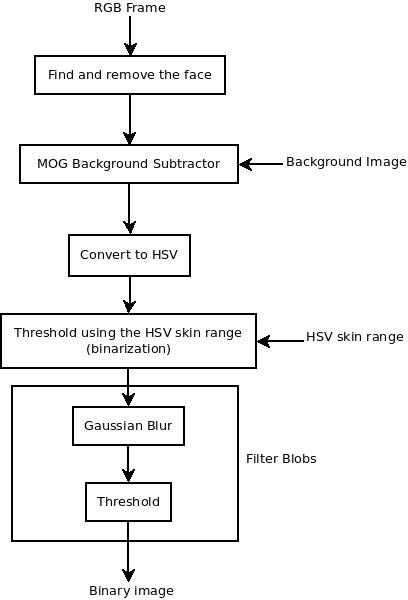
\includegraphics[width=0.4\textwidth]{../images/hand_filter.jpeg} 
\end{figure}
 
As it can be seen in the diagram, the first thing done is to detect the face using the ``Face Detection using Haar Cascades'' already implemented and trained in OpenCV. It is a very reliable clasifier because of the huge dataset used in the training phase. It was used this one instead of making our own in order to have a reliable detector without spending too much time on it, as is just a small part of the segmentation. 


After the face detection, a binary mask is made in which a black square is drawn over the face to hide it.

Next, a Mixture of Gaussians background subtractor is used to remove the background of the image and detect more easily the hand. From this step, another binary mask is created and applied to the original image. 
The background subtractor is inherited from the class cv::BackgroundSubtractorMOG2 made in order to modify the protected parameter ``backgroundRatio''. This parameter measures the frequency at which the background image is updated. In this code, the backgroundRatio is a very low number to make the background update as low as possible. This allows the user to keep the hand in the same position for a while without being recognized as background.  

Afterwards, the resulting image with the latter masks being applied is converted to the HSV color space and is thresholded using the appropriate HSV skin range.
This skin range can be modified at the begining of the program, selecting the theoretical range or calculating a custom range from a skin color sample. Also, is is possible to manually adjust the minimum and maximum HSV values in another window before starting the gesture recognition. 

\begin{center}
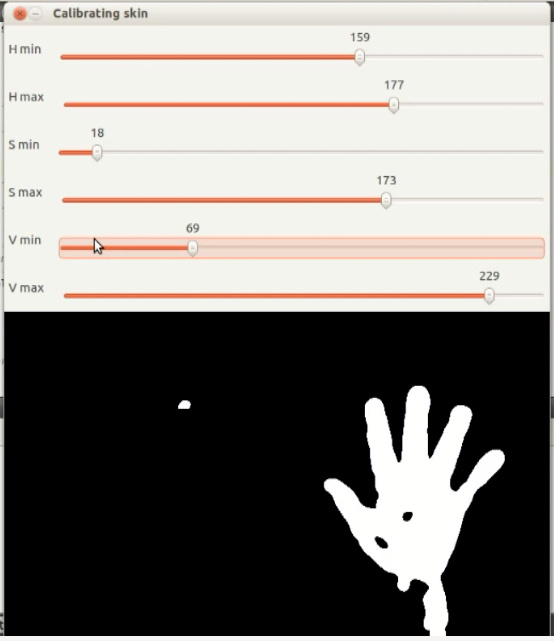
\includegraphics[scale=0.5]{images/threshold.png} 
\end{center}

Finally, in order to better the output binary image, a gaussian blur and a thresholding is applied to eliminate blobs and unite different regions of the hand. It was chosen this configuration because it was much faster and gave better results than making an opening to the image. 

 
\subsection{Hand Description}

The input of this section is the binary image that was the output of the previous one. This part of the software characterizes and extracts the hand parameters. 

\begin{figure}[H]
	\centering
	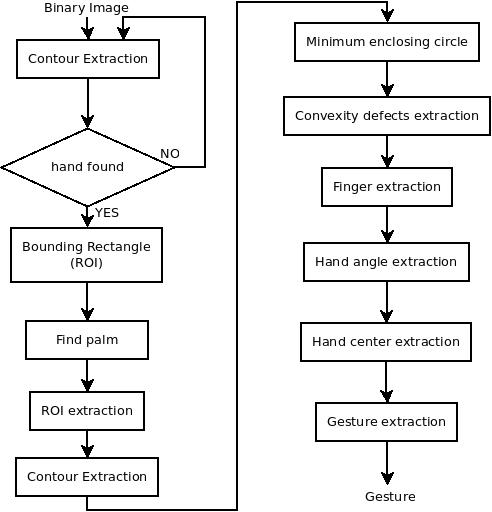
\includegraphics[width=0.5\textwidth]{../images/hand_description.jpeg} 
\end{figure}


The first step is to find all the contours on the binary image, and discard the ones that are too small, as they are likely noise blobs on the image. Once the small contours are filtered, a polygon approximation is carried out to make the contour smaller and reduce the computational load of the algorithm.

If a contour large enough is found, it calculates the bounding box of the contour and the minimum rotated rectangle bounding the contour, for the later angle calculation. Then, the maximum inscribed circunference, that describes the hand palm, is found by calculating the point which maximizes the distance to the hand contour (the inscribed circle center), and its distance (the inscribed circle radius).

The hand is supposed to be inside a circunference of 3.5 times the radius of the maximum inscribed circunference, so we extract that region of interest and find the contours again inside that region, to eliminate any contour due to the forearm skin. The minimum enclosing circunference for that contour is found, which will be used for closed fist / open palm gesture detection.
\begin{center}
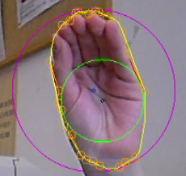
\includegraphics[scale=1]{images/click_cropped.png} 
\end{center}
For the finger detection, the first step is to calculate the convex hull of the hand contour, and then find the convexity defects, the points of the original contour between the vertex of the convex hull that are the furthest away from the hull segment. Each of that defects will represent the valley between two potential fingers, but before they can be considered fingers they have to fulfill three conditions:

\begin{enumerate}
\item The depth of the convexity defect must be in between the minimum bounding circunference radius and the maximum inscribed circunference radius. 
\item The angle between the segments joining the defect depth point and the defect start/end points that represents the angle between two consecutive fingers, must be lower than 90º.
\item The last condition is related to the k-curvature, that should be lower than 70º. The k-curvature is the angle between two segments joining a point close to the fingertip and a point of the contour k places before and after that point. For our software, the value of k chosen was 9, but if the contours used had more points one should increase this value. This condition allows us to find the fingerprint points more accurately.
\end{enumerate}

Those points that fulfilled these three conditions and that were close enough were considered as the same fingerprint.

\begin{center}
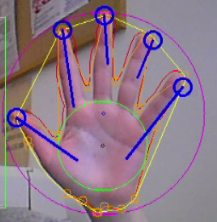
\includegraphics[scale=0.7]{images/5fingers_cropped.png} 
\end{center}

This method works very well with most of the gestures except for the case when the hand has only one finger shown, as the resultant contour will not have any hull defect that accomplishes these conditions.

Next, the angle and center of the hand are extracted and filtered using a Kalman filter, for smoothing the output values and getting a more constant cursor trajectory that allows the user to select buttons and GUI controls more precisely.

Finally, the gesture of the hand is guessed based on the hand descriptors previously extracted. The gestures implemented in this version are:

\begin{itemize}
\item {\bfseries Open palm:} number of fingers found is either 4 or 5.
\item {\bfseries Closed fist:} no fingers were detected, the ratio between the minimum enclosing circunference radius and the maximum inscribed circunference radius is less than 2.
\item {\bfseries Victory sign:} two fingers found, angle between them less than 60º.
\item {\bfseries Gun sign:} two fingers found, angle between them more than 60º (and less than 90º).
\item {\bfseries No gesture found:} The descriptors extracted do not match any of the previous conditions.
\end{itemize}

\hspace{-1.6cm}
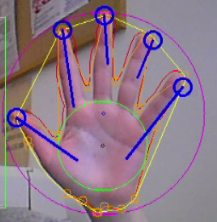
\includegraphics[scale=0.65]{images/5fingers_cropped.png} 
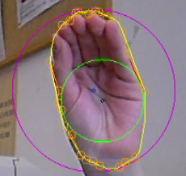
\includegraphics[scale=0.82]{images/click_cropped.png} 
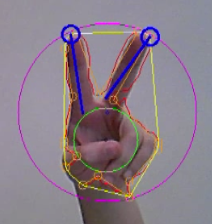
\includegraphics[scale=0.65]{images/victory_cropped.png}
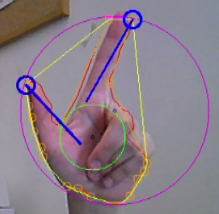
\includegraphics[scale=0.68]
{images/Lgesture_cropped.png} 

Those gestures are encoded using a integer value and used by other parts of the software.


\subsection{Gesture Interface} 

The gesture interface takes as input the gesture guess data from the previous hand description stage, and triggers several actions depending on the gesture and the configuration selected. Due to the presence of false positives and false negatives in the output of the previous stage, and as it could trigger unwanted actions on the computer, a simple state machine is implemented to assure that the program triggers these actions only when they are desired by the user.

The state machine has two states, ``found'' and ``not found'', representing the cases in which the gesture has ocurred or it has not ocurred yet, respectively. It also has two counters, one counting the number of positive matches with the value to track, and the other the number of consecutive negative matches.

If the number of consecutive negative matches is equal to the maximum value allowed, it resets the positive matches counter. If the the number of positive matches equals the minimum value of positive matches needed, it reaches the ``found'' state, and stays there until it is reseted (either by the user or by the arrival of negative matches). 


This interface allows the user to control the cursor and move it around when a ``open hand'' gesture is detected, and to click with a ``closed fist'' gesture. It also allows to launch two different commands with the remaining implemented gestures, than can be configured with a configuration file.

More information about the configuration file, the gestures and how to use the software in the ``User Guide''. 

\newpage
\section{User Guide}
This code was developed using the following libraries: 
\begin{itemize}
\item OpenCV (v2.4.6.1).
\item X11 (linux native libraries that allows the control of the windows and mouse). 
\end{itemize}
The software was compiled using CMAKE (minimum version 2.8).
\\[0.5cm]
Therefore, those libraries are needed for the correct functioning of the software. 


\subsection{Compile the software [UBUNTU]}

In order to compile the code, there are various options. Here it will be explained how to compile using qt and terminal. 
\\
To open the software as a Qt project, the only thing needed is to open the main CMakeLists.txt (gecko/CMakeLists.txt) with QtCreator. This will parse the whole project. 
Afterwards, press the "build" icon to build the project. 
\\[0.5cm]
The folder structure used is the typical of a CMake project. In order to compile using the terminal follow this steps: 
\begin{enumerate}
 \item Open a terminal in the build directory (gecko/build). 
 \item Enter the command "cmake ..". 
 \item Enter the command "make". 
\end{enumerate}

\subsection{Use the software}
In order to execute the software, press the convinient button of the QtCreator IDE or open a terminal in the bin directory (gecko/bin) and enter the command "./gecko". 

Once the code is compiled and started, a first window will appear with the information about the software. After pressing enter to continue, this menu will pop up: 
\begin{center}
\fbox{
\includegraphics[scale=0.5]{../../img/menu.png} }
\end{center}

\vspace{1cm}
The first option will take the theoretical HSV skin values proposed in [1]. Afterwards, the application will allow us to adjust those HSV ranges to adecuate them to the room's conditions. 
Once all the adjustments are done, pressing ENTER will start the program. 

The second option will pop up a window with a green square in the middle. Place the hand so that the square is in the middle of your palm and press ENTER. The program will automatically calculate the HSV range of your skin. Afterwards you will be able once more to manually adjust those ranges. Pressing ENTER one last time will start the program. 
\\
 
The main program will track the hand and trace two circles, the first one around the palm and the second one surrounding the whole hand. The center of the palm is also shown, as well as the angle described by the hand. 

There are different functionalities implemented in this software. 
\begin{itemize}
\item Open hand(i.e. the program detects the five fingers): the mouse moves with the hand's movement.
\item Closed hand: click.
\item "Victory sign": the gedit text editor is opened.
\item "Gun or L sign": a terminal is opened. 
\end{itemize}

The two last functionalities may be changed using a configuration file named apps.config (gecko/data/apps.config). 
That configuration file contains the following:
\\[0.5cm]
\$gedit\$ 3 \\
\$gnome-terminal\$ 4
\\[0.5cm]
The three refers to the victory sign, and the 4 to the gun or L sign. To change the functionality the only thing needed is to change the programs written between the two dollar signs with the wanted one. 

The user should take into account that when the program recognizes a gesture, a rectangle will appear in the window. In order to filter possible false positives, the user must remain in the same posture until the rectangle is completely filled for the correct execution of the task associated with the gesture. 


\newpage

\section{Software Documentation}
The doxygen generated documentation is available in html format in this webpage: \\
\begin{center}
http://david-estevez.github.io/gecko/
\end{center}

\vspace{0.5cm}\hspace{-0.65cm}
There is also a pdf document called ``GECKO\_ Reference\_ Manual"
\newpage


\section{Bibliography}

[1] H.-S. Yeo, B.-G. Lee, and H. Lim,``Hand tracking and gesture recognition system for human-computer interaction using low-cost hardware'', Multimed. Tools Appl., May 2013.
\\[1cm]
[2] A. Albiol, L. Torres, and E. J. Delp, ``Optimum color spaces for skin detection'', no. 3, pp. 3–5.
\\[1cm]
[3] A. Argyros and M. Lourakis, ``Tracking skin-colored objects in real-time'', Cut. Edge Robot., 2005.
\\[1cm]
[4] V. Vezhnevets, ``A Survey on Pixel-Based Skin Color Detection Techniques'', 1994.




\end{document}